\subsection{Geany - Entwicklungsumgebung}

Nach dem Herstellen der Verbindung zur Raspberry Pi �ber SSH kann die grafische Entwicklungsumgebung Geany gestartet werden.

\begin{console}
	cd ~
	geany &
\end{console}

Soll Geany in Englisch ausgef�hrt werden, obwohl das System auf Deutsch gestellt wurde, so muss man vor dem Start die Variable "`LANG"' auf "`C"' setzen.

\begin{console}
	LANG=C geany &
\end{console}

Nun kann eine Source-Datei geladen oder erstellt werden. Dann kann das Konfigurationsfenster ge�ffnet werden, indem man im Men� \texttt{Erstellen} $\rightarrow$ \texttt{Kommandos zum Erstellen konfigurieren} ausw�hlt.\\
Die Parameter f�r \texttt{Kompilieren} und \texttt{Erstellen} werden bereits anhand der Source-Datei (Extention) vorbelegt. Zumeist m�ssen aber noch Anpassungen vorgenommen werden, um Bibliotheken oder ge�nderte Kompiler verwenden zu k�nnen. Werden zwei Source-Dateien im Projekt ben�tigt, so m�ssen auch beide in der Anweisung vorkommen ("'g++ -o Zieldatei Quelldatei1.cpp Quelldatei2.cpp"'). Es k�nnen Platzhalter mit verschiedenen Funktionen eingef�gt werden. \texttt{\%f} wird durch den Dateinamen der im Editor ausgew�hlten Datei ersetzt. \texttt{\%e} wird durch den Dateinamen ohne Extention der im Editor ausgew�hlten Datei ersetzt.\\   
%f - replaced by the filename of the file selected in the editor when the menu item is selected.
%e - replaced by the same filename but without the last extension.
Was genau bei den Feldern einzutragen ist, wird in den folgenden Beispielprogrammen der einzelnen Programmiersprachen angegeben.\\    

Danach kann das Programm mit der Taste \texttt{Erstellen} erzeugt werden und mit der Taste \texttt{Ausf�hren} in einem Terminal gestartet werden.\\
Die Tastenk�rzel f�r alle Funktionen k�nnen �ber das Men� \texttt{Bearbeiten} $\rightarrow$ \texttt{Einstellungen} $\rightarrow$ \texttt{Tastenk�rzel} vorgegeben werden. Dazu w�hlt man die gew�nschte Aktion aus und dr�ckt die Taste "`�ndern"'. Danach kann man die Taste bzw. Tastenkombination dr�cken, die dann umgehend im Dialog angezeigt wird. Wenn nun die OK-Taste gedr�ckt wird, wird die �nderung �bernommen und das Tastenk�rzel f�hrt in Zukunft die Aktion aus. 
Im Beispiel wurde der Aktion "`Erstellen"' dem Tastenk�rzel bzw. der Taste \framebox{F7} zugewiesen.\\ 
Eine Beschreibung zur Erstellung und Parametrierung eines Projekts kann dem Kapitel \ref{sec:Projekt_LED} \titleref{sec:Projekt_LED} bzw. \ref{sec:Projekt_Ampel} \titleref{sec:Projekt_Ampel} 
entnommen werden.

\begin{figure}[ht]
  \centering
  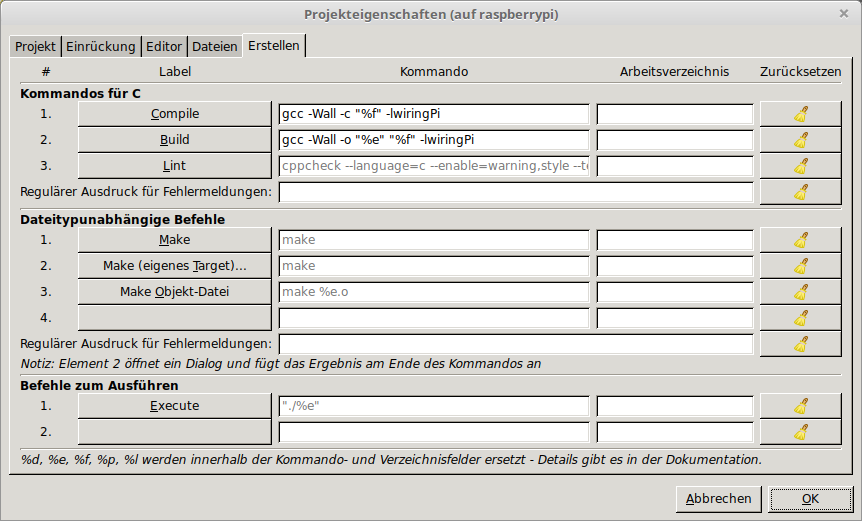
\includegraphics[scale=0.48]{images/Geany_Create.png}
  \caption{Kommandos zum Erstellen konfigurieren f�r C Projekt}
  \label{Geany-create}
\end{figure}

\begin{figure}[ht]
  \centering
  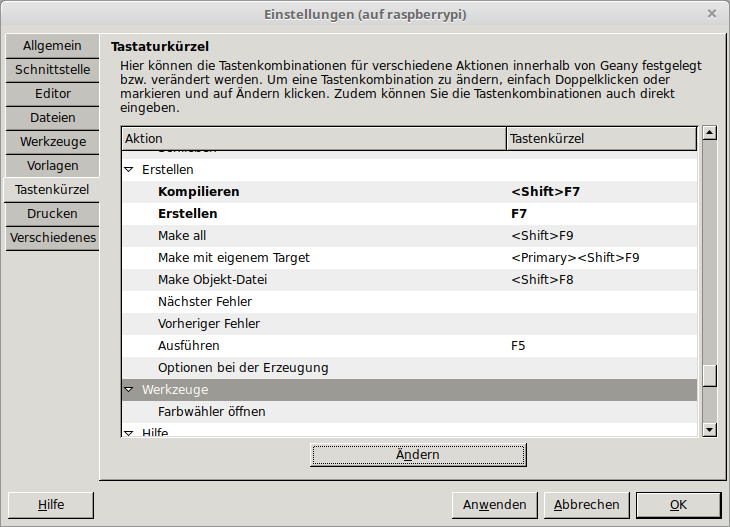
\includegraphics[scale=0.48]{images/Geany_Settings.png}
  \caption{Tastaturk�rzel}
  \label{Geany-settings}
\end{figure} 

\begin{figure}[ht]
  \centering
  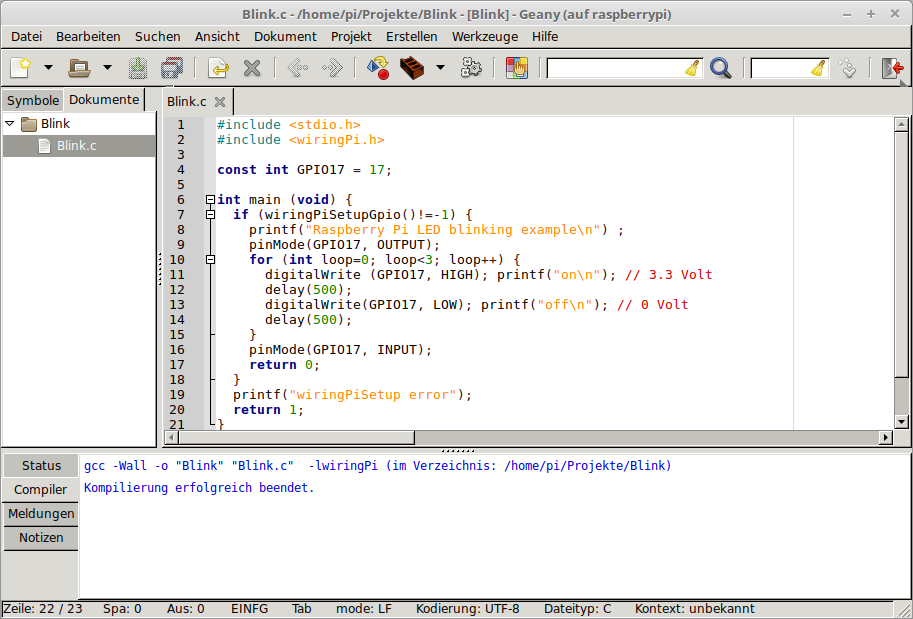
\includegraphics[scale=0.4]{images/Geany_Window.png}
  \caption{Geany Oberfl�che mit Blink-LED Beispiel}
  \label{Geany-window}
\end{figure}
